\graphicspath{ {../body/bayesian_figures/}}
%\chapter{基于连续业务类型的Bayesian博弈分析模型}
%\label{chap_bayesian_game}
\par 
本章的目的是,在用户信息不完备的情况下,通过用户博弈的方式
研究用户类型对无线资源分配与管理的影响。
我们首先提出一个新的业务类型描述方式。
与以往的离散业务类型描述方法不同,我们将用户的业务类型描述成一个连续的随机变量。
然后建立了一个基于Bayesian博弈的竞争与决策分析模型。
这个模型可以有效地描述在不完备信息下的用户资源竞争的情况。
通过理论分析来研究用户的业务类型对博弈结果的影响。
通过理论分析得知,建立适当的收益与惩罚机制,可以激励用户根据自身的业务情况做出理性的分析和决策;既可以保证自身的服务质量,
又能让资源得到充分利用。
%
\section{引言}
由于无线资源稀缺,研究者在无线资源分配及管理方面做了许多意义的工作。
近年来,博弈论做为经济学家常用的数学方法也被引入到无线网络技术研究领域,
特别是针对Ad Hoc网络或无线传感器网络\cite{Srivastava:2005}\cite{FangBensaou2004}。
博弈论的本质是通过数学模型来研究多个利益冲突的理性个体如何调整自己行为的理论。
通过构造合适博弈论模型及其博弈规则,可以引导自私但又理性的个体做出既有利于自已又利于其他参与者的决策。
例如,在多媒体码率分配问题中,用户往往为了保证自身最佳的服务质量,会过多地占用系统的资源,
进而导致整个系统性能的下降。
为此,学者Zhang和Liu针对这个问题,提出竞价博弈及相应的税制机制来限制用户这种过分贪婪的行为\cite{ZhangLiu2011}。

但是,这些方法都通常会有一个比较严格的假设:
在这类博弈中,每个博弈参与者或用户都要具有其他参与者或用户的完备信息。
并且,在博弈过程中,设置一个集中控制的单元负责传递用户之间的各种信息。
例如,在文献\cite{ZhangLiu2011}中,用户的各种私有信息,收益函数的参数等等都要在用户之间进行交换。
这样会导致大量的信息在用户之间传送。
这类博弈分析模型称之为完备信息下博弈模型。
通常,在博弈论研究中,所有参与者知识完备的假设是一个简单而又恰当的近似。
在有些实际的问题中,这种假设过于理想和完美。
例如,根据用户业务类型来进行网络资源分配的问题。
因为随着移动互联网的发展,用户业务种类越来越多,越来越细致。
所以,想在资源分配之前,通过集中控制单元准确获取所有用户对资源的精确需求比较困难。
博弈论中有这样一种类型的博弈:一些参与者可能不知道其他参与者的收益。
这种类型的博弈被称之为“不完全信息的博弈”,或者被称为“Bayesian博弈”。

在本章中我们利用这种新的分析模型:Bayesian博弈分析模型,对系统中参与者的行为进行引导。
这种分析模型与完备信息博弈模型不同。
每个用户除了对自身的情况一清二楚之外,对参加博弈的其他用户的信息并不十分了解。
也就是说他所得到的其他用户信息是不完整的;或是说,每个用户的私有信息是受到一定程度的保护。

\section{业务类型与系统博弈模型}
\subsection{离散与连续的业务类型}
目前,绝大多数的文献对于用户业务的类型讨论都是基于离散的分类形式。
例如,在早期的无线GSM网络中,话音几乎是唯一的业务。
随着网络技术的发展,除了话音外,文字、图片和视频等数据业务相继出现。
不同阶段的通信标准也根据其特点,规定了业务的种类。
比如,3GPP定义了四种基本业务类型,即会话类业务、流媒体业务、交互类业务和背景类业务。
IEEE802.16e中定义了这五种业务类型:UGS,rtPS,ertPS,nrtPS,BE。
在分类的原则上,有的的分类是指从应用层的角度来看待网络承载的数据,例如视频或声音。
有的分类是从网络传输的角度来看。不同的业务类型代表了不同业务对网络性能的要求,如对带宽、时延等等。
假设业务分类可以从概论论的角度来看,那么用户所承载的业务类型的一切可能的结果(离散的)也就可以组成的集合是一个样本空间~$\Omega$~,
那么空间中元素就可以对应为目前网络传输中的一种业务类型定义。

然而,我们如果仔细思考就会发现,这种离散的业务分类方法是有很大的局限性:过于笼统。
譬如,对于同一个视频片段,不同的编码器(MPEG4,H.264,H.265)或同一种编码器的不同编码设置参数都会对视频流的结果产生影响。
对于物理层调制编码,不同的信道模型和编码方法也同样会对传送的数据产生影响。

所以,我们认为除了原有的离散式的业务类型定义以外,还可以将这种离散式分类方法推广到连续式的业务分类方法。
这可能更接近业务本来的面目。
在连续的情况下,业务类型其实是一个概率意义上的随机变量~$X$~,并且服从某个概率分布~$F(x)$~。
每一种现实存在的业务类型都可以对应这个随机的变量的一个取值。
下面我们将这种业务分类连续定义思想应用到Bayesian博弈的分析模型中,并考察业务类型对博弈结果的影响。

\subsection{博弈模型}
假设在一个无线网络基站的覆盖范围内,目前有~$N$~个在线用户正在共享无线资源进行通信。
为了能够更加公平且有效的使用资源,基站控制器会在有新的用户进入的时候,
触发一次资源调整的方案。调整的目的是让用户根据目前自身的业务情况,重新申请合适的资源数量,
避免一些用户长期大量占用资源。
例如,在IEEE802.16标准中,
基站控制器可以通过引导各个用户投票来竞争所需要的资源。
但是由于资源有限,随着用户的数目逐渐增多,竞争就会加剧。
有时会出现先接受服务的用户为了保证自身的服务质量,申请多于自身需求资源且不加以释放。
如果对这种贪婪用户的情况不能有效地加以处理,那么结果会让整个系统的资源利用率恶化。
为了能从机制上规范所有用户的资源使用行为,改变其自身的资源过多占用策略。
我们希望通过Bayesian博弈的方式,引导用户根据自身真实的需求进行理性的资源申请和使用。

对于我们博弈模型,我们首先做如下的假设:
\begin{itemize}
    \item 假设博弈参与者业务类型可以与“参与者成本”相对应。也就是说,我们使用“参与者成本”这个随机变量来表征参与者的业务类型特征。
    \item 假设代表参与者成本的随机变量是独立同分布的,并且其累积概率分布函数~$P(\cdot)$~在区间~$[C_{\min}=0, C_{\max}=1]$~是连续增函数,
    \item 假设每个参与者自身的成本的具体取值是私有的知识,其他的参与者并不知道。
    这里需要注意是,参与者虽然不知道其他参与者成本随机变量的具体数值,但是知道这个随机变量的分布函数。
    之所以做这样假设的原因是,在实际中我们是通过统计的方法获得参与者类型的概率分布。这个信息是公共知识。
    \item 假设模型中的参与者的收益函数也是公共知识。这个信息被所有博弈参与者提前广播通知到的。
\end{itemize}

整个资源分配的过程分成两个步骤。
第一步,是用户选择与博弈阶段。
资源分配单元要征求所有~$N$~个博弈参与者的意见,是否参与本次的资源分配调整过程。
每个参与者都要在这个博弈过程中做出这样的决策:是否同意根据目前自身的情况,只分配最低限度的资源占用数量,从而释放出剩余的资源。
相应的,参与者有两种选择:“慷慨”(Generosity)或是“自私”(selfishness)。
如果选择“慷慨”,系统将按他的所需要的最低资源需求量进行配给。
如果选择“自私”,系统将按他目前申请的资源需求量进行配给。
第二步,资源分配的实施过程。资源分配单元按照参与者在第一步的决定分配物理意义上的无线资源,如带宽或子信道。

首先,我们定义博弈的策略。
显然,参与者在第一步中的选择是关键。
这种选择形式是典型的~$0-1$~决策。
对于任意一个参与者而言,他的策略选择可以用变量~$s_i$~来描述,如\eqref{eqn:chap_bayesian_strategy_definition}所示。
\begin{align}
    s_i = \begin{cases}
        1, \qquad\text{慷慨}\\
        0, \qquad\text{自私}\\
    \end{cases}
    \label{eqn:chap_bayesian_strategy_definition}
\end{align}
其中,此函数的定义域是成本区间~$[C_{\min}, C_{\max}]$~,值域是集合~$\{0,1\}$~中取任意一个值。
“~$1$~”表示参与者愿意“慷慨”;“~$0$~”表示参与者“自私”;
~$i$~表示参与者的序号索引。

然后,我们定义博弈中的参与者收益。
从前面的叙述中可知,在资源有限的情况下,这种博弈本质是一种零和博弈。
每一个自私的参与者希望别的参与者选择“慷慨”,
而自身选择“自私”,不改变目前资源的占用数量。
如果有参与者~$i$~选择“慷慨”,那么我们认为其他选择“自私”的参与者都会因他的“慷慨的行为”而获益~$b=1$~。
而这名博弈参与者所得的收益为~$b-c_i= 1-c_i$~。
显然在此情况下,选择“慷慨”的参与者收益要小于选择“自私”的参与者收益。
但是,为了鼓励参与者选择“慷慨”而且研究选择“慷慨”的参与者数目对博弈结果的影响,我们做如下的假定:
如果选择“慷慨”的参与者数目小于$m$; 其它的参与者都选择“自私”,
不愿意“牺牲”自己的利益,那么所有参与者的获益都将是~$b$~为~$0$~。

那么,对于参与者~$i$~来说,他的收益函数定义为\eqref{eqn:chap_bayesian_player_payoff}:
\begin{equation}
 u_i(s_i, s_{-i}, c_i, m) = s_i\cdot (1 - c_i) + (1-s_i) \cdot \Phi(s_{-i},m)
\label{eqn:chap_bayesian_player_payoff}     
\end{equation}
其中,记号~$-i$~表示除参与者~$i$~之外的其它所有参与者。
记号~$s_{-i}$~表示其他参与者~$-i$~的策略选择集合。
~$c_i$~表示参与者~$i$~的成本。
~$\Phi(s_{-i},m)$~表示对于其他的参与者,是否有~$m$~个参与者选择“慷慨”,如\eqref{eqn:chap_bayesian:m_users_agree}定义所示。
\begin{align}
    \Phi(s_{-i,},m) = \begin{cases}
        1, \qquad \text{if } \sum s_{-i} \ge m;\\
        0, \qquad \text{others};
    \end{cases}
    \label{eqn:chap_bayesian:m_users_agree}
\end{align}

%
\section{Bayesian博弈分析}
对于每一个理性且自私的博弈参与者,他总想通过自己的选择来使自己的收益最大化。
可以表示为~$\max(u_i)$~。
对于所有参与者的选择来说,最后的纯策略均衡可以用一个策略向量~$( s_1^*(c_1^*),\ldots, s_N^*(c_N^*) )$~来描述。
其中,策略~$s_i^*(c_i^*)$~使得~$u_i$~达到最大值。

但是,如果直接求解收益最大化,会使问题本质变成是一个$N$目标优化的极其复杂问题,这是我们所不希望看到的。
所以,为了避免陷入这样情况,我们转而求解参与者的期望收益最大化问题,~$\max\{E(u_i)\}$~。
最后求解出所谓的混合策略。混合策略是纯策略上的一种概率分布。每个博弈参与者的随机化及其他参与者的随机化是统计独立的。
相应的Bayesian博弈的解就是博弈参与者选择“慷慨”或“自私”的概率。

下面我们来具体分析这个博弈。
首先我们引入一个均衡概率的定义~$\theta_{-i}(m)$~。
它表示对于参与者~$i$~而言,至少有~$m$~个其他的参与者的决定是“慷慨”的概率。
实际上,通过这个概率定义的引入,我们使得博弈参与者~$i$~的决策与其它博弈参与者的决策行为相关联。
这样,参与者关于其它参与者的判断可以由自己的收益函数来决定。
同时,也可以看作是,通过这个定义来表征参与者之间的博弈行为。
这个概率的具体表达式如\eqref{eqn:chap_bayesian:at_least_one_probability}所示。
\begin{equation}
    \theta_{-i}(m) = \hbox{Prob} \Bigl\{ \Phi( s_{-i},m) = 1 \Bigr\}, \, m\le N-1
    \label{eqn:chap_bayesian:at_least_one_probability} 
\end{equation}
所以,对于一个给定的博弈参与者~$i$~,他的期望收益可以由\eqref{eqn:chap_bayesian_player_payoff} 
和\eqref{eqn:chap_bayesian:m_users_agree}定义为如下公式:
\begin{align}
     E(u_i) &= \theta_{-i}(m)\left[s_i(b-c_i) +(1-s_i)\right] \notag \\
     & \quad + [1-\theta_{-i}(m)] [s_i(b-c_i) + 0] \notag\\ 
     &= s_i[1-c_i-\theta_{-i}(m)] + \theta_{-i}(m)
    \label{eqn:player_expe_payoff}
\end{align}

从\eqref{eqn:player_expe_payoff}可以看出,为了使得~$E(u_i)$~尽可能大,并考虑决策的前提下,可以分成两种情况。
如果博弈参与者~$i$~的成本~$c_i$~小于~$1-\theta_{-i}(m)$~,那么参与者~$i$~的决策就是“慷慨”,也就是~$s_{i}=1$~。
如果~$c_i > 1 - \theta_{-i} (m)$~,那么参与者~$i$~会选择“自私”,~$s_i = 0$~。
那么我们也将其写为一个分段函数的形式。
\begin{align}
    s_i(c_i) = \begin{cases} 
        1, &\text{if $c_i < 1 -\theta_{-i}(m)$;}\\
        0, &\text{if $c_i > 1 -\theta_{-i}(m)$.}\\ \end{cases} 
    \label{eqn_equilibrium_strategy} 
\end{align}
从\eqref{eqn_equilibrium_strategy}可以看出,参与者~$i$~的成本对决策的影响很关键。
如果他的成本~$c_i$~在区间~$ [C_{\min}, c_i^*] $~,参与者的决策就是“慷慨”。
其中,我们把~$c_i^*$~称为均衡临界成本。
所以,参与者~$i$~选择“慷慨”概率,也就是均衡临界成本的概率~$P(c_i^*)$~,
如\eqref{eqn:chap_bayesian:equil_prob_c_i}所示。
\begin{align}
    P(c_i^*) = \hbox{Prob} \Bigl\{ C_{\min} < c_i \leq c_i^* \Bigr\} 
    \label{eqn:chap_bayesian:equil_prob_c_i}
\end{align}
而且,
%因为对于每一个博弈参与者而言,他的业务随机变量或成本随机变量而言,是独立同分布的。
因此,如果存在这样一个均衡临界成本,
%可以将~$\theta_{-i}(m)$~看作为一个二项分布的情况。
我们将\eqref{eqn:chap_bayesian:equil_prob_c_i} 代入\eqref{eqn:chap_bayesian:at_least_one_probability},
那么就有:
\begin{align} 
    \theta_{-i}(m) &= \hbox{Prob} \Bigl\{ \Phi( s_{-i},m) = 1 \Bigr\} \notag \\ 
   % &= C_{N-1}^m [P(c^*)]^m [1-P(c^*)]^{N-m-1} \notag \\
   % & \quad + \cdots + C_{N-1}^{N-1} [P(c^*)]^{N-1} [1-P(c^*)]^{N-(N-1)-1} \notag \\
   % &= \sum_{k=m}^{N-1}C_{N-1}^k [P(c^*)]^k [1-P(c^*)]^{N-k-1}
   &= P(c_1^*)P(c_2^*)\cdots P(c_{m}^*) \cdot (1-P(c_{m+1}^*)) \cdots(1-P(c_{N-1}^*)) \notag \\ 
    & \quad +  P(c_0^*)P(c_2^*)\cdots P(c_{m+1}^*) \cdot (1-P(c_{m+2}^*)) \cdots(1-P(c_{N-1}^*)) \notag \\ 
    & \quad + \cdots  + P(c_1^*)P(c_2^*)\cdots P(c_{N-2}^*) \cdot (1-P(c_{N-1}^*)) \notag \\
    & \quad +  P(c_1^*)P(c_2^*)\cdots P(c_{N-1}^*)  
    \label{eqn:chap_bayesian:two_poly_distribution}
\end{align}
\eqref{eqn:chap_bayesian:two_poly_distribution}表示了在其它参者个数为~$N-1$~的情况下,
至少存在~$m$~个参与者选择“慷慨”的概率。如果
同时,从\eqref{eqn:chap_bayesian:at_least_one_probability}和\eqref{eqn_equilibrium_strategy}可知,
均衡临界成本 ~$c_i^*$~是用户决策的关键值。它关系到用户选择的转换。
因此,均衡临界成本还要满足下面\eqref{eqn_equilibrium_cost}
\begin{align}
    c_i^* &= 1 - \theta_{-i} (m) \notag \\
     & =1 - [P(c_1^*)P(c_2^*)\cdots P(c_{m}^*) \cdot (1-P(c_{m+1}^*)) \cdots(1-P(c_{N-1}^*)) \notag \\ 
    & \quad +  P(c_0^*)P(c_2^*)\cdots P(c_{m+1}^*) \cdot (1-P(c_{m+2}^*)) \cdots(1-P(c_{N-1}^*)) \notag \\ 
    & \quad + \cdots  + P(c_1^*)P(c_2^*)\cdots P(c_{N-2}^*) \cdot (1-P(c_{N-1}^*)) \notag \\
    & \quad +  P(c_1^*)P(c_2^*)\cdots P(c_{N-1}^*) ]
    \label{eqn_equilibrium_cost} 
\end{align}
对于博弈中的任意一个~$c_i^*, i=1,\ldots, N$~,都要满足
\eqref{eqn_equilibrium_cost}。
又因为所有参与者的成本随机变量是独立同分布的,并且对于每一个~$c_i^*, i=1,\ldots, N$~
在\eqref{eqn_equilibrium_cost}等号左右两边是可以任意互相交换的。
所以对于一种分布来说,那么它们值一定相等,即~$c_1^* = c_2^* = c_3^* \cdots = c_N$~。
则我们把这个值记为~$c^*$~。
因此,我们可以将 \eqref{eqn_equilibrium_cost}改写为二项分布的形式,如
\eqref{eqn:chap_bayesian:equilibrium_cost_equation}所示。我们可以通过解这个方程来计算得出~$c^*$~。
\begin{align}  
    c^* & =  1 - [ C_{N-1}^m [P(c^*)]^m [1-P(c^*)]^{N-m-1} \notag \\
   & \quad + \cdots + C_{N-1}^{N-1} [P(c^*)]^{N-1} [1-P(c^*)]^{N-(N-1)-1} ]\notag \\
   &= 1- \sum_{k=m}^{N-1}C_{N-1}^k [P(c^*)]^k [1-P(c^*)]^{N-k-1}
\label{eqn:chap_bayesian:equilibrium_cost_equation}
\end{align}

综上所述,对于我们提出的Bayesian博弈模型而言,网络中博弈参与者成本(用户业务类型)的概率分布情况会对博弈结果起着关键的影响作用。
%%%%%%%%%%%%%%
\section{不同业务类型概率分布的分析与讨论}
下面,我们假设博弈参与者成本(业务类型)为两种最常见的概率分布形式,并分别对其进行分析与讨论。
\subsection{均匀分布的情况}
均匀分布是连续概率分布函数中最常见和最简单的。它在所有的概率分布中占着重要的地位。
许多实际上重要的随机变量者服从或是近似服从均匀分布。
此处,我们假设参与者的类型的概率分布~$P(\cdot)$~是在区间~$[C_{\min}=0, C_{\max}=1]$~上的均匀分布。
它的概率密度函数为
\begin{align}
    f(c) = \begin{cases} c, &\text{if ~$c \in [C_{\min}=0, C_{\max}=1]$~;}\\
        0, &\text{others}\\ 
    \end{cases} 
    \label{eqn_equilibrium_prob} 
\end{align}
其中,我们假设对于参与者的成本被认为是归一化的。
概率密度函数与分布函数图形如\figref{fig:chap_bayesian:uniform_density_scheme}和\figref{fig:chap_bayesian:uniform_cdf_schem}所示。
%%%%%%%%%%%%%%%%%%%%%%%%%%%%%%%%%%%%%%%%%%%%%%%%%%%%%%%%%%%%%%%%%%%%%
\begin{figure}[tb] 
  \begin{minipage}[t]{0.5\linewidth} 
    \centering 
    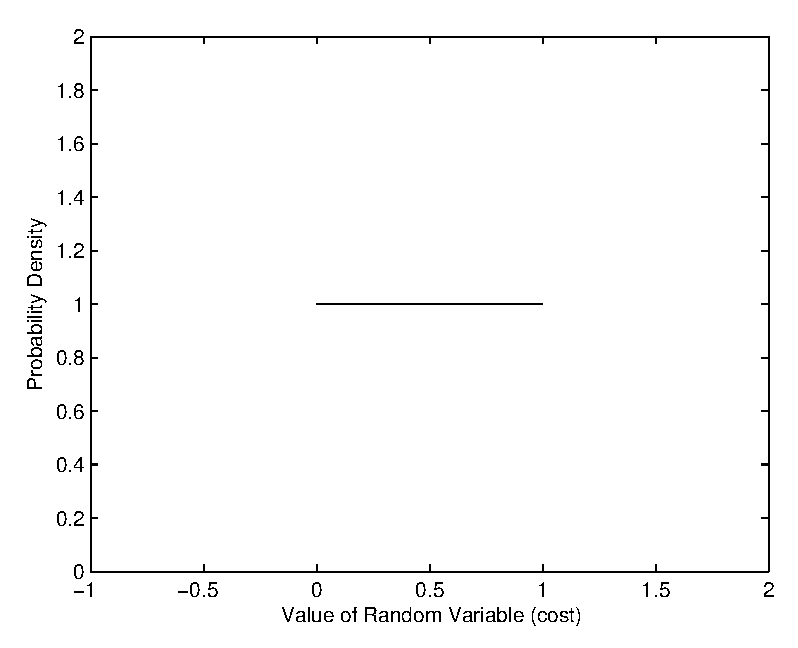
\includegraphics[width = \textwidth]{bayesian_uniform_density_scheme.eps} 
    \caption{均匀分布的概率密度函数} 
    \label{fig:chap_bayesian:uniform_density_scheme} 
  \end{minipage}% 
  \begin{minipage}[t]{0.5\linewidth} 
    \centering 
    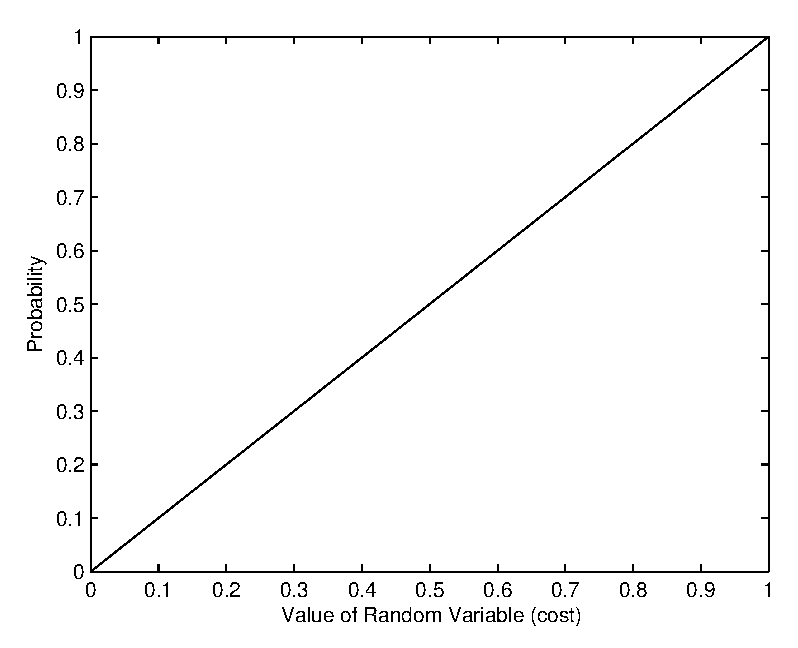
\includegraphics[width=\textwidth]{bayesian_uniform_cdf_scheme.eps} 
    \caption{均匀分布的累积概率函数} 
    \label{fig:chap_bayesian:uniform_cdf_schem} 
  \end{minipage} 
\end{figure}
则达到临界成本~$c^*$~来说,选择“慷慨”的概率为
\begin{align} 
    P(c^*) &= \text{Prob} \Bigl\{ 0 < c_i < c^*\Bigr\} \notag\\ 
    &= \frac{c^*}{C_{\max}-C_{\min}} \notag\\
    &= c^* 
    \label{eqn_probability_of_contribution} 
\end{align}
把\eqref{eqn_probability_of_contribution}代入\eqref{eqn:chap_bayesian:equilibrium_cost_equation}则有
\begin{align*} 
    c^* = 1- \sum_{k=m}^{N-1}C_{N-1}^k (c^*)^k [1-(c^*)]^{N-k-1}
\end{align*}

我们通过做图的方式来直观地讨论在均匀分布的情况下,各个参数对于临界成本和参与者决策的影响,
如\figref{fig:bayesian_user_numb_vs_contr_prob}所示。
%如\figref{fig:bayesian_user_numb_vs_contr_prob}和\figref{fig:bayesian_puni_para_vs_cont_prob}所示。
图中所涉及的奖励~$b$~,成本~$c$~都是归一化后的,且为了简单起见,~$b = 1$~。
%%%%%%%%%%%%%%%%%%%%%%%%%%%%%%%%%%%%%%%%%%%%%%%%%%%%%%%%%%%%%%%%%%%%%
\begin{figure}[tb]
\begin{centering}
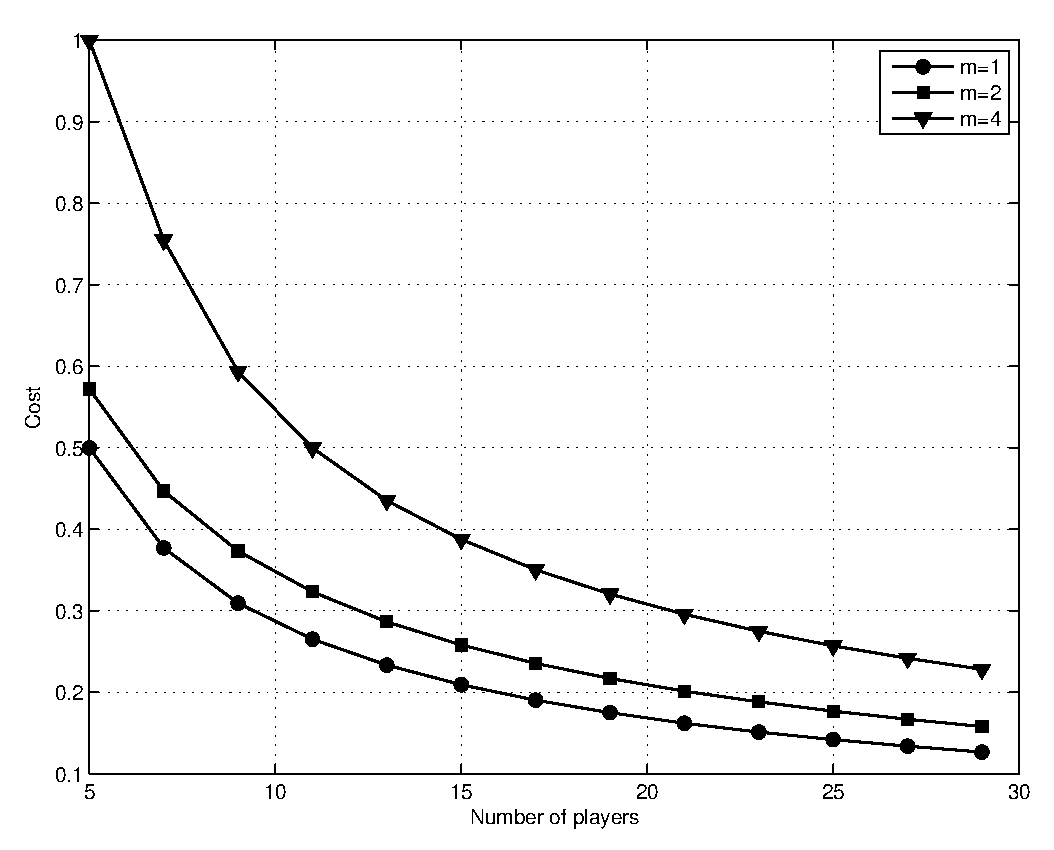
\includegraphics[scale=0.6]{bayesian_uniform_user_number_vs_contribute_probability.eps}
\caption{参与者数目与临界成本的关系(均匀分布)}
\label{fig:bayesian_user_numb_vs_contr_prob}
\end{centering}
\end{figure}
%%%%%%%%%%%%%%%%%%%%%%%%%%%%%%%%%%%%%%%%%%%%%%%%%%%%%%%%%%%%%%%%%%%%
%%%%%%%%%%%%%%%%%%%%%%%%%%%%%%%%%%%%%%%%%%%%%%%%%%%%%%%%%%%%%%%%%%%%%
%\begin{figure}[tb]
%\begin{centering}
%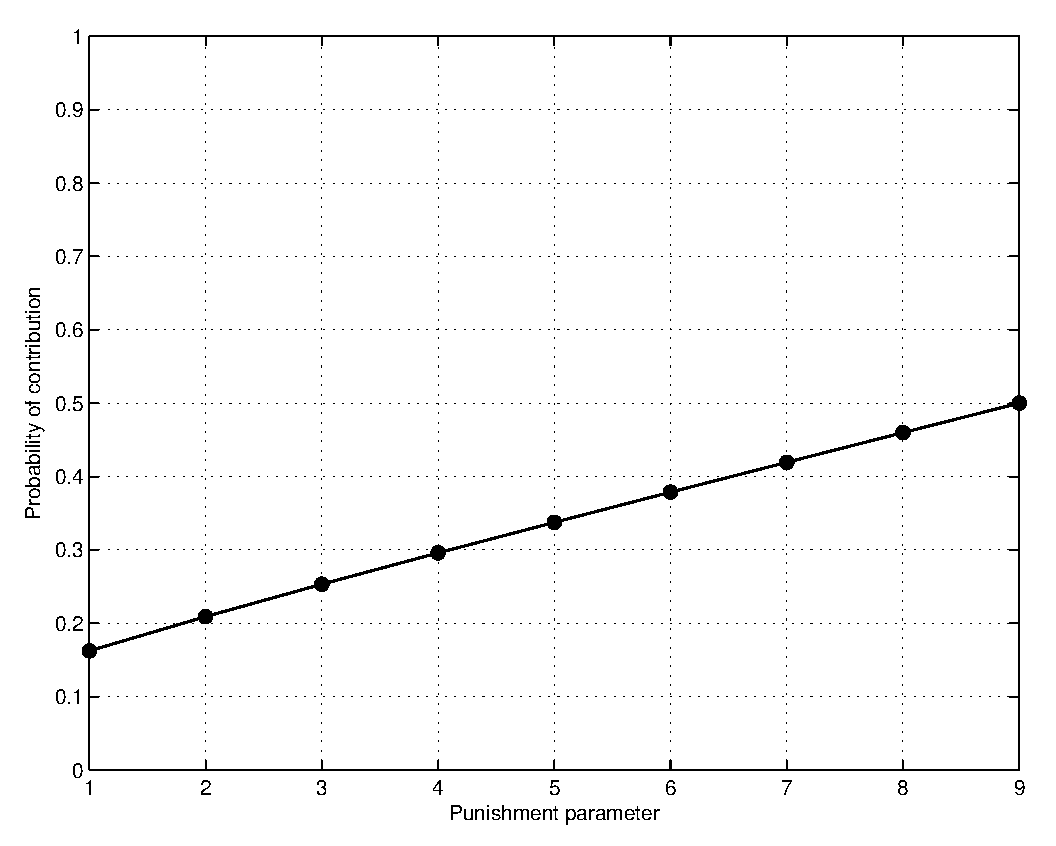
\includegraphics[scale=0.7]{bayesian_uniform_punish_parameter_vs_contribute_probability.eps}
%\caption{“慷慨”参与者数目最低要求$m$与临界成本的关系(均匀分布),$N=10$}
%\label{fig:bayesian_puni_para_vs_cont_prob}
%\end{centering}
%\end{figure}
%%%%%%%%%%%%%%%%%%%%%%%%%%%%%%%%%%%%%%%%%%%%%%%%%%%%%%%%%%%%%%%%%%%%
从\figref{fig:bayesian_user_numb_vs_contr_prob}可以看到,
当博弈的参与者总数增多时,临界成本~$c^*$~会减小。
前面我们提到,当博弈参与者的成本~$c_i$~在区间~$ [C_{\min}, c_i^*] $~,参与者的决策就是“慷慨”。
因而,最终博弈均衡中选择“慷慨”的概率~$P(c_i^*)$~也会随之降低。
这意味着,当系统中参与者较少时,参与者容易做出接受资源调整的决策。
而当系统参与者较多时,即使参与者的收益比成本高,参与者也可能会做也自私的决定。
这说明,当用户总数目多的情况下,自私的用户都希望他人来做出资源占用的调整,而自身却“自私”调整。
另外,
%从\figref{fig:bayesian_puni_para_vs_cont_prob}
可以看到,当对决策“慷慨”的数目~$m$~有最低要求时,博弈参与者的“自私”决策概率会降低。
因为大家都会担心没有人选择“慷慨”来让自己最终的收益为零。
因此在系统中设置一个能够自适应网络状态的最低“慷慨”的参与者数目,也是调节参与者选择态度的有效手段。

\subsection{正态分布的情况}
对于参与者的成本类型,第二种我们假设的概率分布是正态分布。
也是一个在数学、物理及工程等领域都非常重要的概率分布。
对于参与者成本随机变量~$c$~服从一个位置参数为~$\mu$~,尺度参数为~$\sigma$~的概率分布,
通常可以记为:
\begin{align*}
    c \sim N(\mu, \sigma^2)
    %\label{eqn:normal_distribution}
\end{align*}
服从正态分布的随机变量的概率密度函数~$f(x)$~由\eqref{eqn:chap_bayesian:normoal_density}和\eqref{eqn:chap_bayesian:normoal_cdf}给出,
且其概率密度函数和概率分布函数如\figref{fig:chap_bayesian:normal_density_scheme}和\figref{fig:chap_bayesian:normal_cdf_schem}所示。
其中,与均匀分布类似的,为了将成本随机变量控制在区间~$[0,1]$~,我们假设成本概率分布的均值为~$\mu = 0.5$~,方差~$\delta = 0.1$~。
\begin{align}
    f(x) = \frac{1}{\sigma \sqrt{2\pi} } e^{ \frac{-(c-\mu)^2}{2\sigma^2}}
    \label{eqn:chap_bayesian:normoal_density}
\end{align}
\begin{align}
    F(x) = \frac{1}{\sigma \sqrt{2\pi} } \int^x_{-\infty}e^{ \frac{-(c-\mu)^2}{2\sigma^2}}
    \label{eqn:chap_bayesian:normoal_cdf}
\end{align}
%%%%%%%%%%%%%%%%%%%%%%%%%%%%%%%%%%%%%%%%%%%%%%%%%%%%%%%%%%%%%%%%%%%%%
\begin{figure}[tb] 
  \begin{minipage}[t]{0.5\linewidth} 
    \centering 
    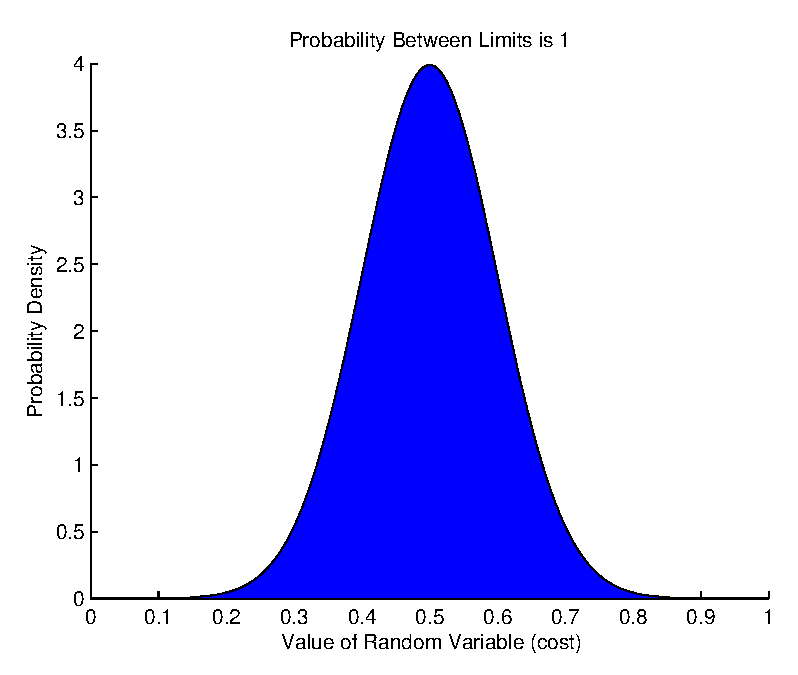
\includegraphics[width = \textwidth]{bayesian_normal_density_scheme.eps} 
    \caption{正态分布的概率密度函数} 
    \label{fig:chap_bayesian:normal_density_scheme} 
  \end{minipage}% 
  \begin{minipage}[t]{0.5\linewidth} 
    \centering 
    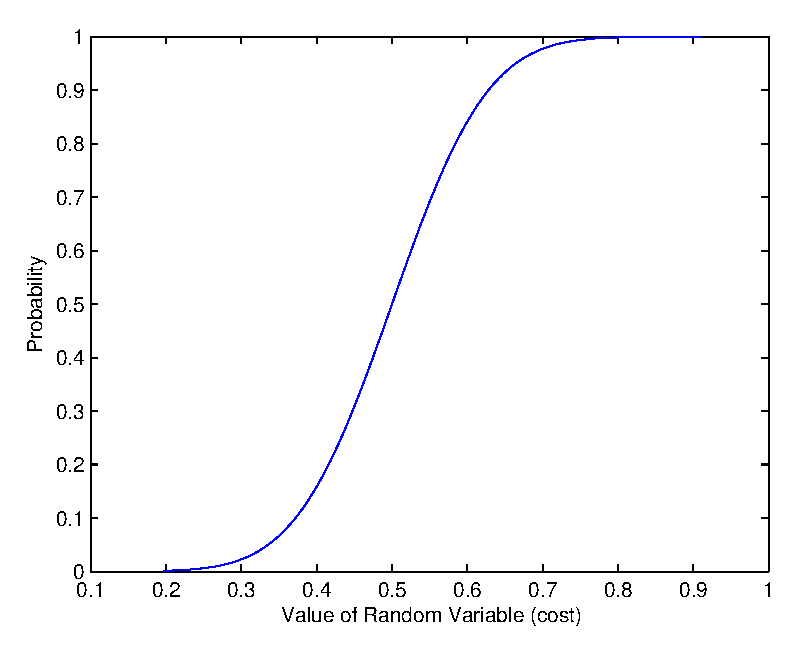
\includegraphics[width=\textwidth]{bayesian_normal_cdf_scheme.eps} 
    \caption{正态分布的累积概率函数} 
    \label{fig:chap_bayesian:normal_cdf_schem} 
  \end{minipage} 
\end{figure}
类似的,如果将\eqref{eqn:chap_bayesian:normoal_cdf}代入\eqref{eqn:chap_bayesian:equilibrium_cost_equation},
则有,
\begin{align} 
    c^* &= 1- \sum_{k=m}^{N-1}C_{N-1}^k \left\{\left[ \frac{1}{\sigma \sqrt{2\pi} } \int^x_{-\infty}e^{ \frac{-(c^*-\mu)^2}{2\sigma^2}})\right]^k \right. \notag \\
    & \qquad \left. \quad \cdot \left[1- \frac{1}{\sigma \sqrt{2\pi} } \int^x_{-\infty}e^{ \frac{-(c^*-\mu)^2}{2\sigma^2}}\right]^{N-k-1} \right\}
     \label{eqn:chap_bayesian:cost_normal_distribution_equation}
\end{align}
由于正态分布函数概率密度函数不能显式积分,所以我们只能通过数值求解的方式,将收益参数、“慷慨”人数最低值、参与者数目与均衡成本关系画出来。
如\figref{fig:bayesian_normal_user_numb_vs_contr_prob}和\figref{fig:bayesian_normal_puni_para_vs_cont_prob}所示。
%%%%%%%%%%%%%%%%%%%%%%%%%%%%%%%%%%%%%%%%%%%%%%%%%%%%%%%%%%%%%%%%%%%%%
\begin{figure}[tb]
\begin{centering}
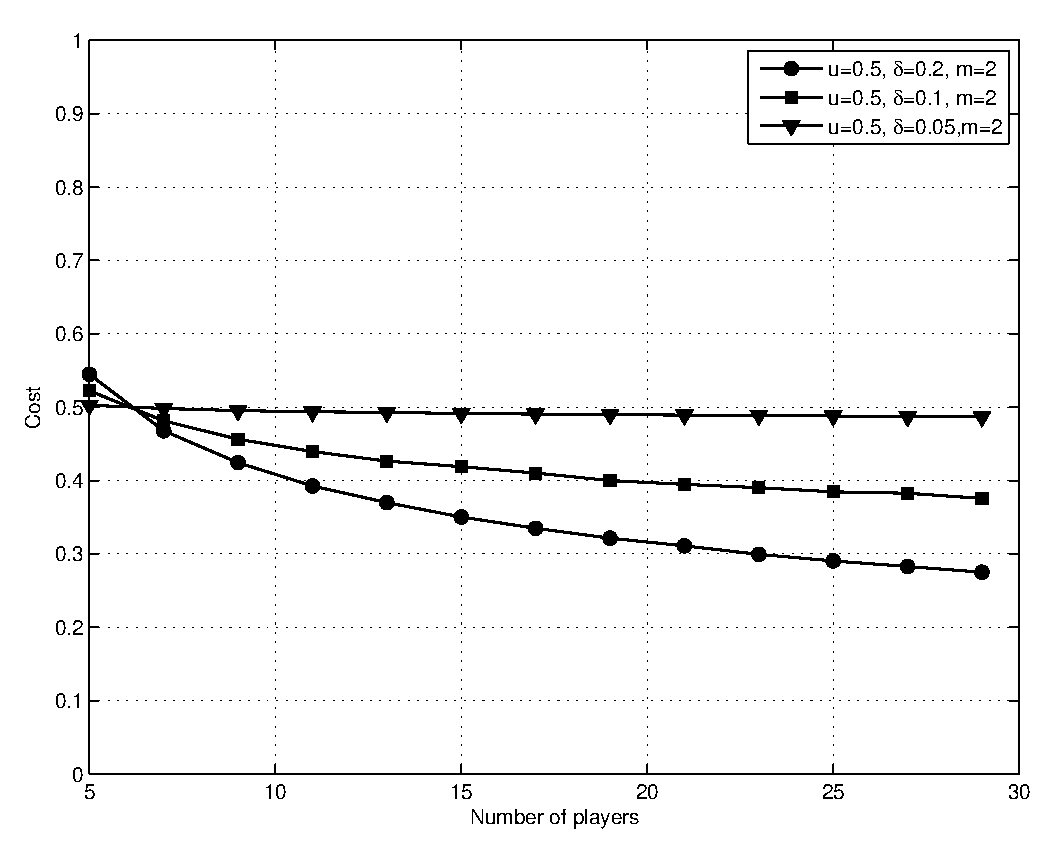
\includegraphics[scale=0.6]{bayesian_normal_user_number_vs_contribute_probability.eps}
\caption{参与者数目与临界成本的关系(正态分布)}
\label{fig:bayesian_normal_user_numb_vs_contr_prob}
\end{centering}
\end{figure}
%%%%%%%%%%%%%%%%%%%%%%%%%%%%%%%%%%%%%%%%%%%%%%%%%%%%%%%%%%%%%%%%%%%%
%%%%%%%%%%%%%%%%%%%%%%%%%%%%%%%%%%%%%%%%%%%%%%%%%%%%%%%%%%%%%%%%%%%%%
\begin{figure}[!tb]
\begin{centering}
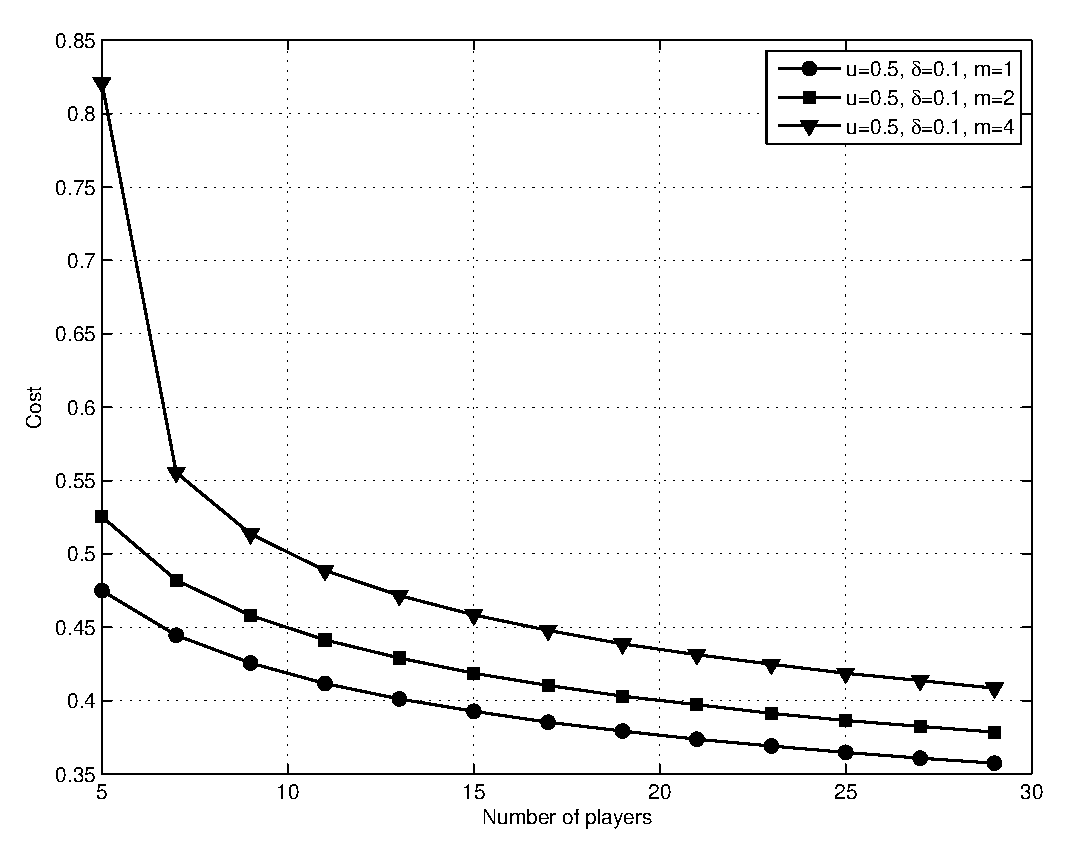
\includegraphics[scale=0.6]{bayesian_normal_punish_parameter_vs_contribute_probability.eps}
\caption{“慷慨”参与者数目最低要求$m$与临界成本的关系}
\label{fig:bayesian_normal_puni_para_vs_cont_prob}
\end{centering}
\end{figure}

与均匀分布的情况十分相似,
当博弈的参与者总数增多时,临界成本~$c^*$~会减小, 如\figref{fig:bayesian_normal_user_numb_vs_contr_prob}如示。
同样,博弈参与者选择“慷慨”的概率~$P(c_i^*)$~也会随之降低。
同理,当系统中参与者较少时,参与者容易做出接受资源调整的决策。
我们还绘制了正态分布的尺度参数~$\delta$~对临界成本的影响。
当尺度参数的取值较小时,意味着博弈参与者的类型分布集中比较集中。
从图中可以看出,用户类型集中的情况下,博弈参与者选择“慷慨”的概率也较高。
\figref{fig:bayesian_normal_puni_para_vs_cont_prob}也表明,
当对“慷慨”参与者的数目的最低值增大时,参与者决策均衡中“慷慨”的机率会增大。这一点与均匀分布一样。

\section{基于博z弈的自适应业务分布资源分配算法}
至此,我们解决了在资源不足以致于不可能给每一个博弈参与者提供最好服务质量下,
让博弈者自己来决定可以降低自己的资源需求。

根据前面的分析,本节我们提出一个资源分配算法来满足每一个用户的需求。
资源分配单元,当有用户要申请更多的资源时,收集各个参与者的业务类型或成本信息。
根据预设的分布模型,将成本信息汇总以后,进行参数估计,求得均值与方差。
然后确定这一时间段内的分布函数的具体形式,并广播给当前服务区的用户。
用户收到本时段的分布函数后,可计算出当前的均衡成本值。
然后用这个值作为选择“慷慨”的概率,做出自身的决策。
最后将决策报告给资源分配单元,完成实际的分配工作。

此分配算法的具体流程如 算法 \ref{alg:chap_bayesian:agr_cac} 所示。
\begin{algorithm}[!ht]
\SetAlgoLined
% assume $B_{ava}=0$\;
等待用户申请资源 \;
如果某一个用户$i$根据自己的当前成本~$c_i$~提出新的资源申请要求$b_i$ \;
\eIf {当前空闲资源可满足用户$i$的需求}{
通知“资源控制分配单元”,给用户申请所需的资源 \; 
}{
向当前服务的所有用户广播“成本收集”消息 \;
所有用户向 “资源控制与分配单元” 报告自己当前的成本 \;
“资源控制与分配单元”选择预设的成本随机分布模型 \;
对模型中参数进行参数估计(均值或方差) \;
将业务模型及刚才得到的参数估计广播给所有用户 \;
每个用户得到业务模型后,计算均衡成本$c^*$及选择“慷慨”的概率 \;
按照“慷慨”的概率值做出自己的最后决策\;
\eIf{决策为“慷慨”}{
    向资源控制与分配单元报告自己的决策和自己对资源最低要求\;
    }
    {
    向资源控制与分配单元报告自己的决策和自己目前的资源需求\;
    }
资源控制与分配单元接收到所有的回复报告\;
统计用户总的需求与目前总的资源\;
\eIf{用户总需求$\le$总资源供给}{
    本次资源调整成功\;
    \For{$k=1$ \KwTo $N$}{
    给每一个在线用户分配资源\;
    }
    }{
    此次资源调整失败\;
    并通知用户$i$\;
    }
    本次资源调整结束\;
}
    转到 \bf 1\;
\caption{基于博弈的自适应业务分布资源分配算法} 
\label{alg:chap_bayesian:agr_cac}
\end{algorithm}

\section{仿真实验与分析}
为了验证我们进行的理论分析结果,以及提出的分配算法有效。
我们参照基站分配资源的基本功能设计以下仿真模型。
在这个仿真模型中,包括一个资源控制与分配单元和$N$个用户。
这$N$个用户符合某个预设的业务类型分布模型,每个用户的慷慨成本为$c_i$。
每个用户的对资源的需求假设带宽$b_i$,在64Kbps到4Mbps之间取值;
并且,因为$c_i$是对用户而言要付出的成本,所以为了简单起见,假设每个用户对资源的最低需求为$(1-c_i)b_i$。

为了验证理论分析,我们编写了第一个仿真的脚本。
同样,我们比较两种业务分布函数,均匀分布和正态分布。
其中,正态分布的参数设置为$\mu = 0.5, \delta^2 = 0.1$;
最少参与者决策“慷慨”的数目设置为$m=4$。
为了能够得到一个统计意义的结果,仿真脚本每组运行了$300$次。
最后的仿真结果如
\figref{fig:chap_bayesian:normal_bandwidth_vs_user_number}至
\figref{fig:chap_bayesian:normal_bandwidth_vs_withdraw_bw}
所示。
%%%%%%%%%%%%%%%%%%%%%%%%%%%%%%%%%%%%%%%%%%%%%%%%%%%%%%%%%%%%%%%%%%%%%
\begin{figure}[tb] 
   \begin{minipage}[t]{0.5\linewidth} 
    \centering 
    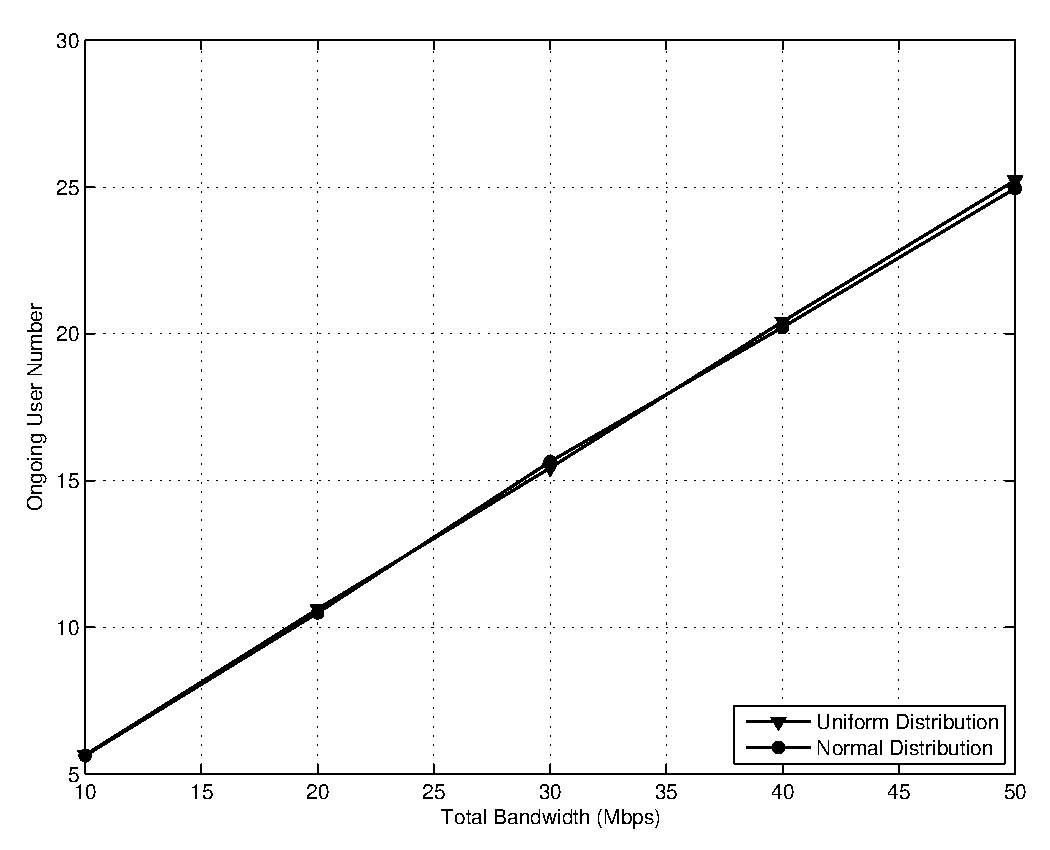
\includegraphics[width = \textwidth]{bayesian_normal_bandwidth_vs_user_number} 
    \caption{在线用户数目} 
    \label{fig:chap_bayesian:normal_bandwidth_vs_user_number} 
  \end{minipage}% 
  \begin{minipage}[t]{0.5\linewidth} 
    \centering 
    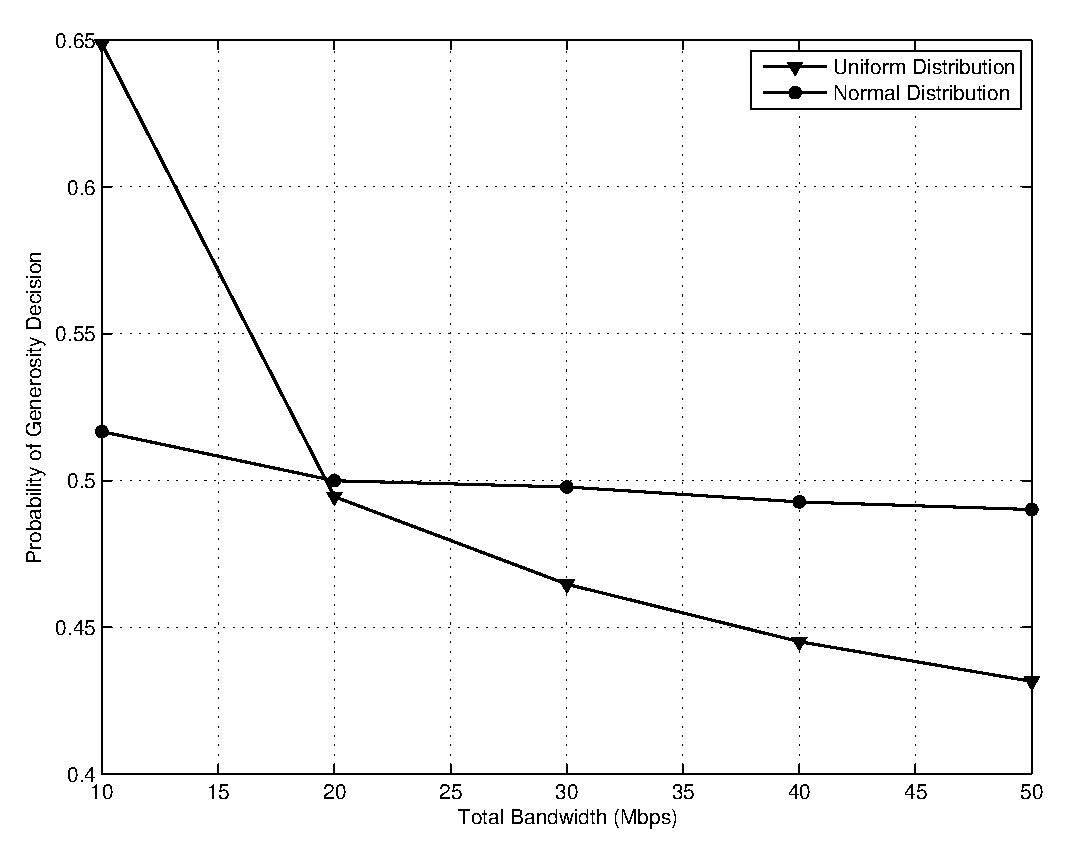
\includegraphics[width = \textwidth]{bayesian_normal_bandwidth_vs_generosity} 
    \caption{用户决策“慷慨”概率} 
    \label{fig:chap_bayesian:normal_bandwidth_vs_generosity} 
  \end{minipage}% 
\end{figure}

\begin{figure}[tb] 
 \begin{minipage}[t]{0.5\linewidth} 
    \centering 
    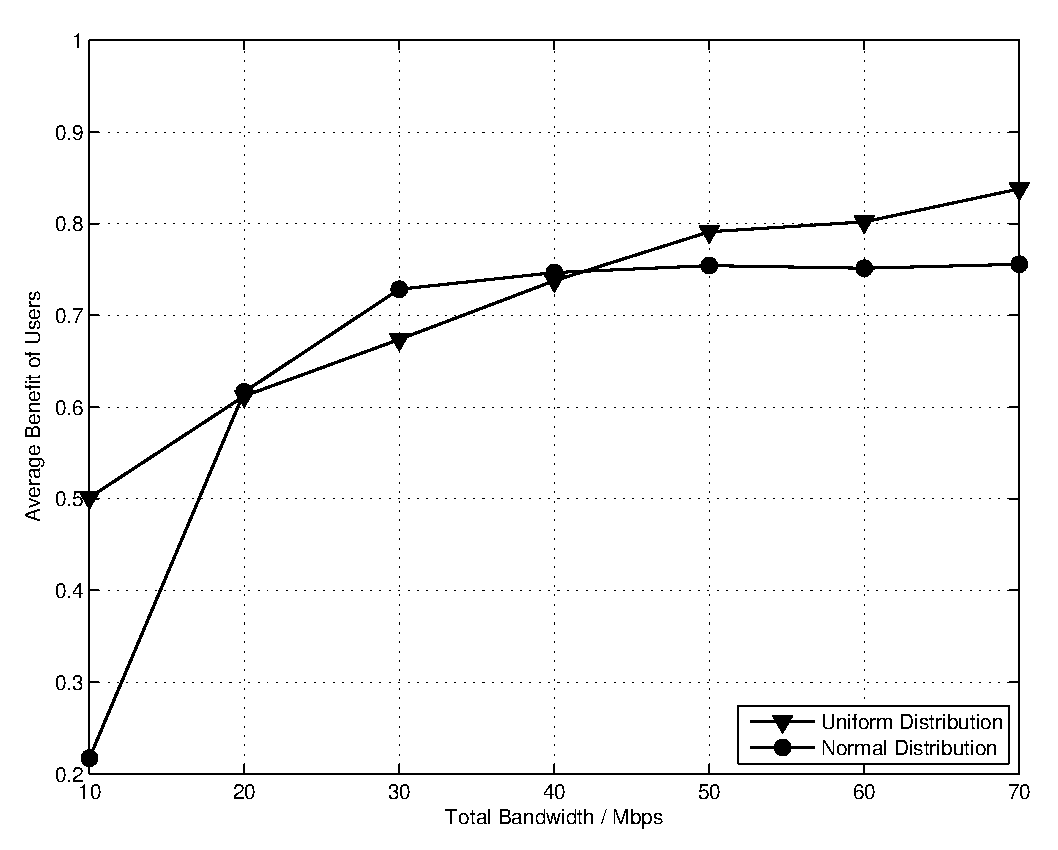
\includegraphics[width = \textwidth]{bayesian_normal_bandwidth_vs_avg_benefit.eps} 
    \caption{用户平均收益} 
    \label{fig:chap_bayesian:normal_bandwidth_vs_avg_benefit} 
  \end{minipage}% 
  \begin{minipage}[t]{0.5\linewidth} 
    \centering 
    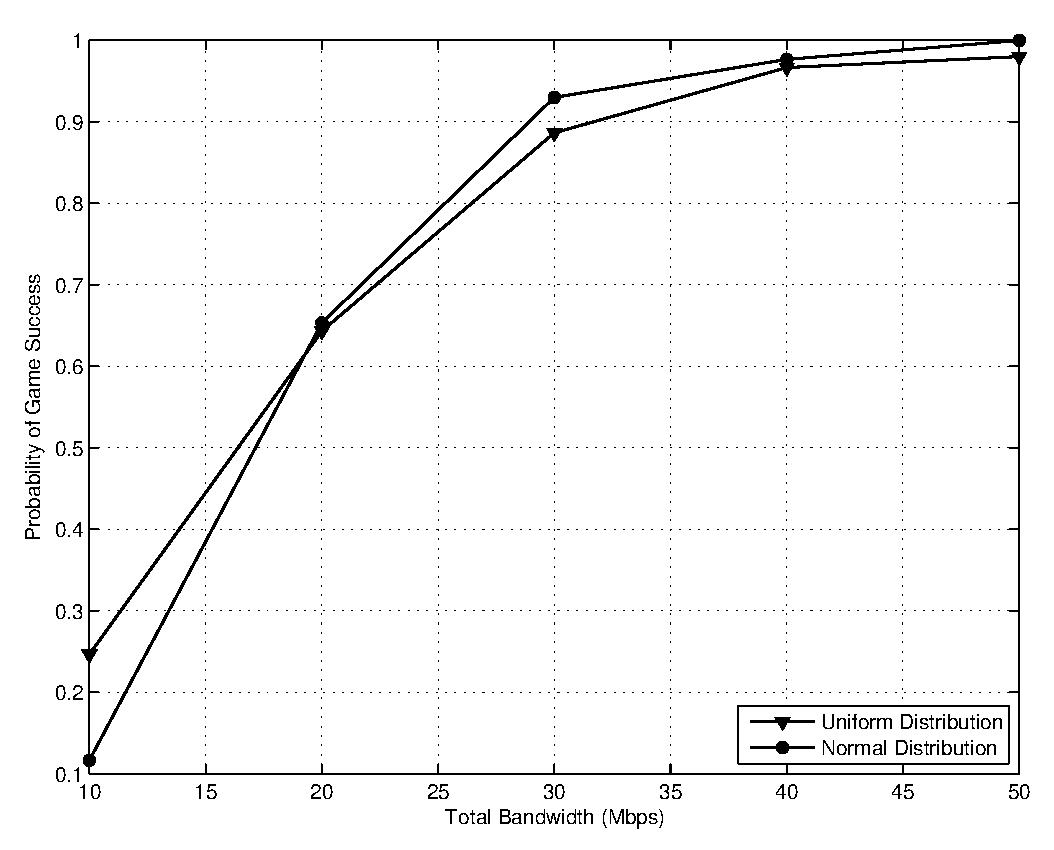
\includegraphics[width=\textwidth]{bayesian_normal_bandwidth_vs_success_probability.eps} 
    \caption{博弈成功概率} 
    \label{fig:chap_bayesian:normal_bandwidth_vs_success_probability} 
  \end{minipage} 
\end{figure}

%%%%%%%%%%%%%%%%%%%%%%%%%%%%%%%%%%%%%%%%%%%%%%%%%%%%%%%%%%%%%%%%%%%%%
\begin{figure}[tb] 
    \centering
  \begin{minipage}[t]{0.5\linewidth} 
    \centering 
    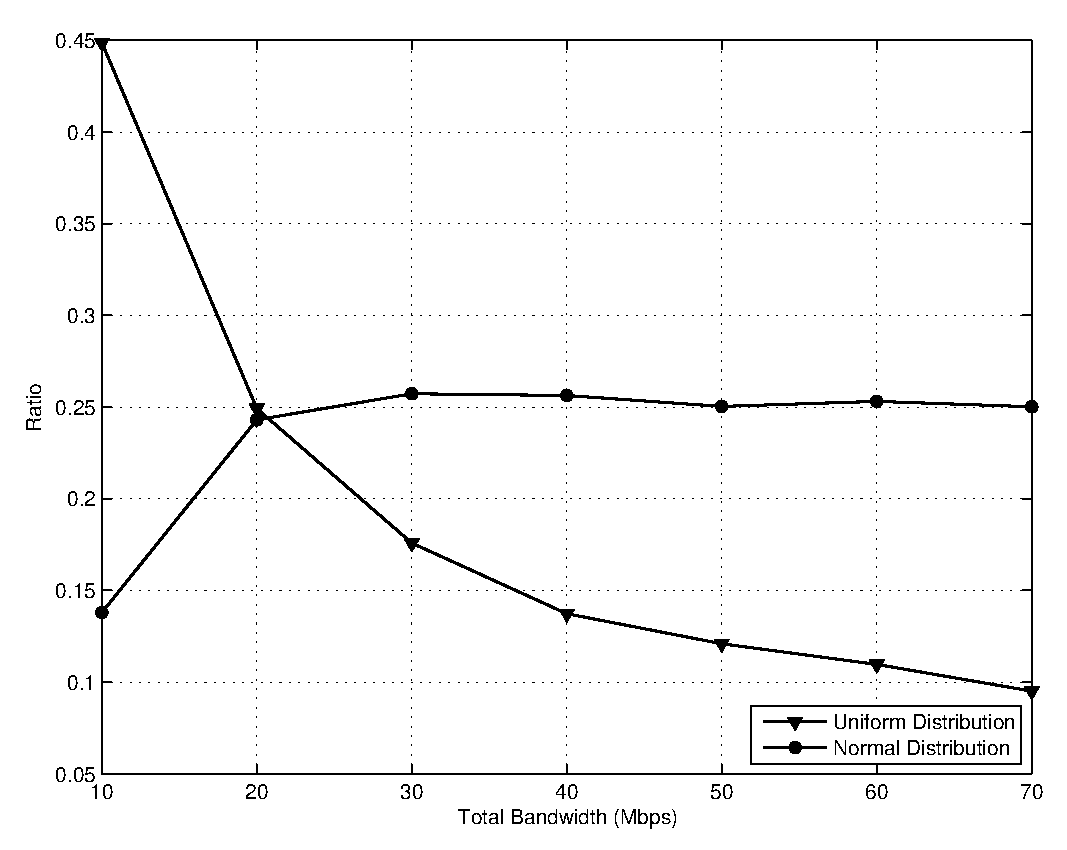
\includegraphics[width=\textwidth]{bayesian_normal_bandwidth_vs_withdraw_bw.eps} 
    \caption{回收资源占总资源的比率} 
    \label{fig:chap_bayesian:normal_bandwidth_vs_withdraw_bw} 
  \end{minipage} 
\end{figure}
仿真脚本通过改变系统的资源总量,来观察博弈结果的变化情况。
很明显,从\figref{fig:chap_bayesian:normal_bandwidth_vs_user_number}可以看出,资源总量的变化首先影响的是在线用户的数目。
系统总带宽的增多,很自然可以容纳更多用户。
与理论分析相同,单个用户决策“慷慨”的概率降低,\figref{fig:chap_bayesian:normal_bandwidth_vs_generosity}所示;
但同时,我们从
\figref{fig:chap_bayesian:normal_bandwidth_vs_avg_benefit}、
\figref{fig:chap_bayesian:normal_bandwidth_vs_success_probability}中可以看到,
用户的平均收益和一次博弈成功概率都会增多。
这里,“一次博弈成功概率”是指在一次博弈过程中,至少有$m$个参与者愿意减少自己占用资源的数量的概率。
用户的数目多少对于博弈的结果影响很大。
从单个用户的角度看,参与者数目增多会使得单个参与者选择“慷慨”的概率下降,
单个参与者从自己的利益出发,更希望其它的参与者选择“慷慨”而自身选择“自私”的情况下还能得到收益。
但是,从集体的角度看,用户数目的增多会弥补这一问题。
这说明,用户数目增多会激发集体的“理性”在更大程度上发挥作用,
在保证在线用户基本满意的前提下使系统本身受益:收集更多“空闲”资源放入空闲资源池中,供新来用户使用,如\figref{fig:chap_bayesian:normal_bandwidth_vs_withdraw_bw} 所示。

第二个仿真脚本,是对分配算法的一个模拟。
这个脚本可从时间维度上观察所提出的博弈分配算法在一个基站中起的作用。

\subsection{用户情境}
\subsection{时间正常情境}

\section{小结}
本章针对网络中业务逐渐增多的趋势,提出通过概率连续随机变量来描述用户的业务类型。
与传统的离散分类不同,新的方法可以更加细致地刻化用户业务特征。
并且根据网络的实际情况,我们提出在不完备信息的情况下通过构造Bayesian博弈模型的方法来寻求使得所有用户满意的资源分配混合策略。
通过理论的分析与仿真实验证明,所提出的业务描述方法及博弈算法,为有效地解决在多用户竞争下的资源分配问题提供另外一条新的途径。


